\chapter{配置应用环境}\label{ch:remote}
\index{Yuancheng jisuan@远程计算}

完成本地结构和工作流练习后，可以按需要调整界面、连接材料数据库，或把计算提交给已经配置好的远程环境。这些功能分别解决不同的问题：设置决定应用如何与个人服务配合，远程计算决定工作流在哪里执行，日志与帮助则用于理解当前状态并交流问题。

本章先介绍日常使用的设置与对话服务，再介绍完整 MATLAB\regmark{} 工具箱中的远程提交。节点内的CPU、进程池与GPU设置见第\ref{sec:node-resources}节；本章的远程部分解决的是把任务交给哪一个计算环境。使用独立应用或基于 Runtime 的在线版时，可按自己的部署条件使用节点资源，并阅读设置、对话、日志与帮助各节。

\section{调整应用设置}

\subsection{打开设置并保存修改}

在 \ui{主页} 的环境区域点击 \ui{设置}。通用页包含界面语言和对话服务设置，Materials Project 页用于数据库访问；连接账号服务的在线版环境还提供账号页。

更改后点击 \ui{确认} 才会保存。点击 \ui{取消} 或直接关闭设置窗口，会放弃本次尚未确认的修改。再次打开窗口时，会重新读取已经保存的值，可以据此核对实际采用的设置。

\subsection{切换界面语言}
\index{Jiemian yuyan@界面语言}

\begin{steps}
\item 打开 \ui{主页 → 设置 → 通用}。
\item 在语言区域选择需要的界面语言。
\item 点击 \ui{确认}，保存选择。
\item 保存正在编辑的项目，然后重新启动应用。
\item 检查工具栏与面板标题是否已经使用新的语言。
\end{steps}

语言在下次启动时生效。桌面应用关闭后重新打开即可；在线版中 \ui{退出 KSSOLV Toolbox} 只是暂时返回入口，原实例仍在运行。在线版用户需要先保存项目，再按平台的注销或重新启动流程进入新的实例。

图\ref{fig:settings-language-field}给出在线版通用页的语言区域局部。当前选择为简体中文，输入框下方说明语言在下次启动时生效；这与本节先保存设置、再重新启动的操作顺序对应。

\begin{figure}[!htb]
\centering
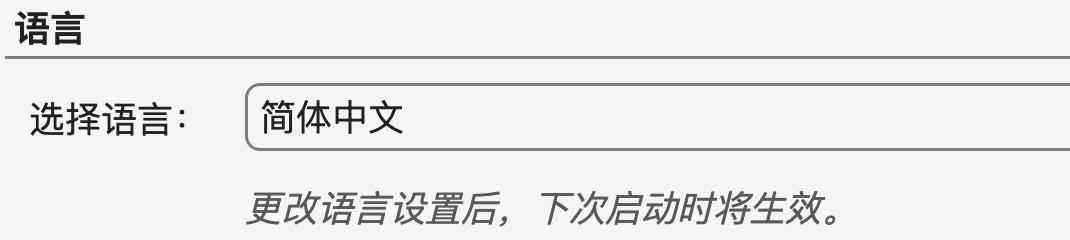
\includegraphics[width=102mm]{publication-assets/crop-290321d16b2310a99270.png}
\caption{设置通用页的语言字段实例，当前选择简体中文。}
\label{fig:settings-language-field}
\end{figure}


\section{连接对话服务}\label{sec:llm-configuration}
\index{Duihua fuwu@对话服务}

\subsection{选择服务类型}

命令行窗口除了执行可用命令，还可以向大语言模型提问。应用提供\ui{OpenAICompatible}与\ui{Ollama}两种服务类型。前者使用OpenAI兼容的接口，由服务提供方给出基础地址、密钥与模型名称；后者连接已经运行的Ollama服务，使用该服务已经安装的模型。

对话适合解释术语、比较参数的用途和整理工作笔记。支持工具调用的模型还可以读取当前工作流、修改节点标签。它不是运行DFT前必须完成的步骤；即使没有配置对话服务，也可以导入结构并执行本书的数值教程。

\begin{table}[!htb]
\centering
\caption{选择服务时需要准备的信息。}
\label{tab:llm-connection-fields}
\begin{tabularx}{\linewidth}{lXX}
\toprule
设置 & OpenAICompatible & Ollama \\
\midrule
地址 & \ui{API 基础地址}，包括提供方要求的版本路径，如\file{/v1}。 & \ui{服务地址}，如本机服务的\url{http://127.0.0.1:11434}。\\
凭据 & \ui{API Key}，填写该基础地址对应的密钥。 & 此设置页不提供API Key字段。\\
模型 & \ui{使用的模型}，选择或输入账号可用的模型标识。 & \ui{使用的模型}，选择或输入服务端已安装的名称与标签。\\
检查 & \ui{测试连接}或刷新按钮获取模型列表。 & \ui{测试连接}或刷新按钮获取已安装模型列表。\\
\bottomrule
\end{tabularx}
\end{table}

这里的地址由运行工具箱的机器访问。桌面应用通常从桌面计算机发出请求，在线版则由服务器或容器访问服务；浏览器所在电脑并不自动成为模型服务的运行位置。

\subsection{设置 \headinglatin{OpenAI} 兼容服务}

开始前，从服务提供方取得基础地址、个人 API Key 和有权使用的模型。这里使用“OpenAI 兼容”指接口形式，实际提供方和模型以账号中可用的服务为准。

\begin{steps}
\item 在 \ui{主页 → 设置 → 通用} 中找到\ui{大语言模型}区域，将\ui{类型}设为\ui{OpenAICompatible}。
\item 在 \ui{API 基础地址} 中输入提供方给出的基础地址，保留其要求的版本路径。
\item 在 \ui{API Key} 中输入个人密钥。
\item 点击 \ui{测试连接}，等待获取模型列表的状态提示。
\item 从 \ui{使用的模型} 中选择可用模型，或按提供方说明输入准确标识，核对名称后点击 \ui{确认}。
\item 回到命令行窗口，用一个简短的概念问题检查服务是否能正常回答。
\end{steps}

图\ref{fig:settings-service-fields}展示OpenAI兼容服务的配置字段。基础地址保留提供方要求的版本路径；模型标识应与服务端可用名称一致。图中只演示字段填写，连接状态需按自己的服务实际检查。

\begin{figure}[!htb]
\centering
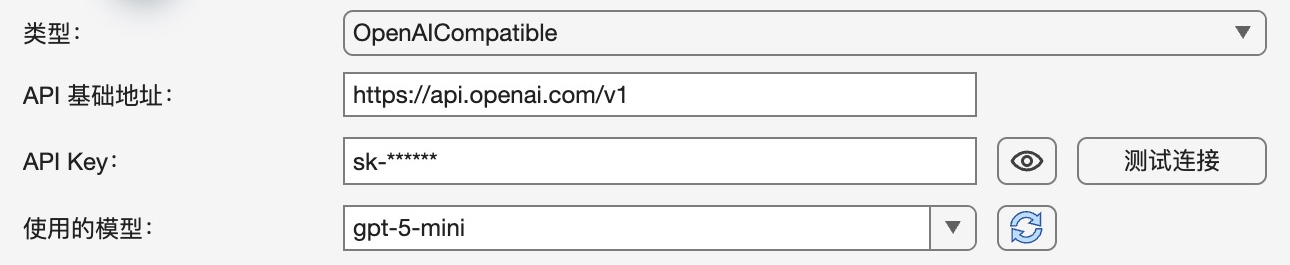
\includegraphics[width=\linewidth]{publication-assets/revision-llm-openai-compatible.png}
\caption{OpenAI兼容服务的中文设置页局部。基础地址、密钥和模型分别填写；密钥以遮挡形式显示。}
\label{fig:settings-service-fields}
\end{figure}

基础地址不要再附加 \file{/chat/completions} 或 \file{/models}，也不要把服务商的网站首页当作API地址。例如，提供方要求的基础地址若以\file{/v1}结束，就应保留这一段；应用随后会自行追加获取模型列表或请求回复的路径。设置页会拒绝已经包含上述具体接口路径的基础地址。

密钥输入框通常以遮挡形式显示。若需更正可以使用显示按钮短暂查看，完成后恢复隐藏。如需删除已经保存的OpenAI密钥，先选择另一种不使用它的服务，再清空密钥并点击\ui{确认}；仍选OpenAI兼容服务时，设置页会要求填写可用密钥。截图或共享屏幕时保持密钥隐藏。

\subsection{设置 \headinglatin{Ollama}}

Ollama 需要一个已经运行并能由应用访问的服务。桌面用户可以使用本机服务，在线版则需使用服务器能访问的地址。浏览器在自己的电脑上，并不意味着服务请求也从这台电脑发出。

\begin{steps}
\item 在\ui{类型}中选择\ui{Ollama}。
\item 在\ui{服务地址}填写服务根地址，不附加\file{/api/tags}或其他具体API路径。本机默认端口的地址可写为\url{http://127.0.0.1:11434}。
\item 点击\ui{测试连接}，等待读取服务端的模型列表。
\item 在\ui{使用的模型}中选择服务已经安装的模型，或输入完整名称与标签，再点击 \ui{确认}。
\item 回到命令行窗口发送简短问题，检查状态与回复。
\end{steps}

在线版中的 \file{localhost}或\file{127.0.0.1} 指运行工具箱的服务器或容器，不能用它指向个人笔记本上的 Ollama。使用统一模型服务时，直接填写部署方给出的服务器地址。在列表中填写模型名称不会替服务器下载模型；模型的安装与服务启动应先在提供该服务的环境中完成。


\begin{figure}[!htb]
\centering
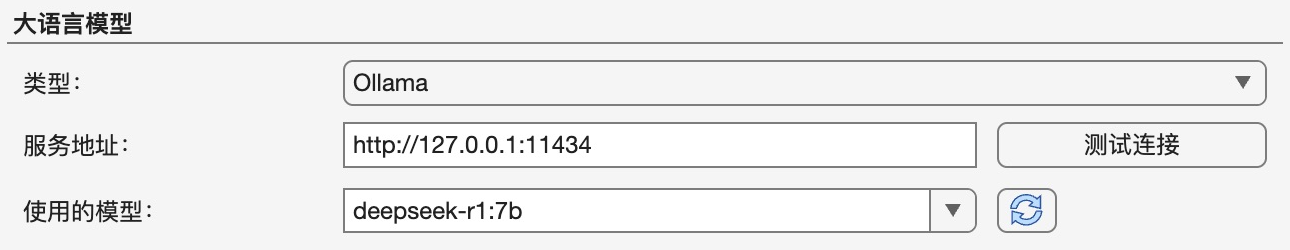
\includegraphics[width=\linewidth]{publication-assets/revision-llm-ollama.png}
\caption{Ollama服务的地址与模型配置。}
\label{fig:llm-ollama-live}
\end{figure}

\subsection{刷新模型列表}

\ui{测试连接}和模型旁的刷新图标执行同一种检查：向当前地址获取模型列表。OpenAI兼容服务读取\file{/models}，Ollama读取\file{/api/tags}。取得非空列表后，状态显示\ui{连接成功，已获取模型}及数量。这里没有发送一条试聊消息，也没有检查某个模型能否完成文本或工具调用。

修改地址或密钥后，先刷新，再检查\ui{使用的模型}。测试期间按钮会改为\ui{停止测试}，点击它可以结束本次等待。模型框允许手动输入，因此当服务没有返回可枚举列表、但提供方另给了准确模型名称时，可以填写该名称并保存，再通过一次简短提问检查对话。此时列表测试仍可能提示没有发现模型，不能把手动填写理解为模型已获验证。

认证失败时检查地址与密钥是否属于同一服务；接口不存在时检查基础地址及版本路径；超时或安全连接提示则检查运行工具箱的机器能否连接该服务。若能取得模型列表但提问失败，继续检查所选模型的使用权限、对话接口以及工具调用支持，而不要只反复刷新列表。界面提示本发行包没有对话组件时，应使用提供相应组件的发行环境；这不会影响本书的结构与DFT教程。

\subsection{在命令窗口提问}\label{sec:chat-use}

对话和普通命令共用一个输入区，由开头符号区分。普通MATLAB\regmark{}表达式直接输入；以一个美元符号开头表示带已有对话上下文提问，以两个美元符号开头表示本次不带已有对话历史。美元符号是输入的一部分，不需要先切换另一张聊天页面。

\begin{table}[!htb]
\centering
\caption{同一输入区中的命令与提问。}
\label{tab:command-chat-prefix}
\begin{tabularx}{\linewidth}{lX}
\toprule
输入示例 & 实际作用 \\
\midrule
\texttt{2 + 3} & 执行MATLAB\regmark{}表达式，在命令窗口显示结果。\\
\texttt{\$}后接问题 & 向模型提问，沿用此前成功完成的对话上下文。\\
\texttt{\$\$}后接问题 & 独立提问，不读取也不追加此前保存的对话上下文。\\
\bottomrule
\end{tabularx}
\end{table}

\begin{steps}
\item 在设置中确认服务与模型后，打开命令行窗口，等待输入区可用。先输入\literalinput{2 + 3}并按Enter，识别普通命令的返回位置。
\item 输入\literalinput{$ 请解释平面波截断能的含义}，按Enter，观察等待状态及逐步出现的回复。
\item 需要继续追问时，输入\literalinput{$ 为什么还需要检查k点收敛}，使问题沿用当前对话。
\item 希望独立询问另一件事时，输入\literalinput{$$ 请说明分数坐标的三个分量}。这不会清空前面的对话；下一次单美元符号提问仍可沿用原上下文。
\item 将需要保留的解释整理到实验笔记，再回到结构或工作流执行真正的建模与计算。
\end{steps}

首次提问时，应用才建立所选服务的对话客户端。发送后观察等待状态与逐步出现的回复，回复结束后状态区可能显示服务实际返回的模型名称。正在回复时，应等这一轮结束再提下一问。

应用可以显示普通文字、代码块和数学表达式。模型写出的代码只是回复内容，不会因为显示在窗口里便自动执行。需要尝试其中某条命令时，先核对变量和输入，再将它作为不带美元符号的普通命令提交。也不要假定模型已经读到了当前结构坐标、图形中的全部数值或项目中的所有文件；需要讨论的条件应在问题中明确写出。


\begin{figure}[!htb]
\centering

\includegraphics[width=108mm]{publication-assets/revision-llm-question-input.png}
\caption{命令窗口中的提问输入示例。开头的美元符号区分对话与普通命令；画面为发送前状态。}
\label{fig:llm-input-live}
\end{figure}

\subsection{让模型查看并整理当前工作流}\label{sec:chat-workflow-tools}

支持工具调用的模型可以请求应用执行两项操作：读取当前工作流的节点与连线，以及修改指定节点的标签。读取当前流程对应\texttt{getCurrentGraph}；修改标签对应\texttt{changeNodeLabel}。这两项工具不负责新建结构、修改计算参数、启动计算或读取整个项目的数值结果。

OpenAI兼容请求会带上这两项工具的定义，服务与模型需要支持相应的工具调用格式。Ollama则根据服务报告的模型能力决定是否提供工具；不支持工具的模型仍可进行普通文本对话。模型是否选择调用工具，要看这一轮实际返回，不能仅凭服务类型推断操作已经执行。

\begin{steps}
\item 保存当前项目，激活一张已经建立的工作流，使其成为当前画布。
\item 输入\literalinput{$ 请读取当前工作流，说明节点标签和连接顺序}。能够调用工具时，模型可用实际流程信息组织回答。
\item 检查回答中的标签是否与画布一致。如果回答只是一般说明，明确要求读取当前工作流；仍没有实际信息时，检查所选模型的工具支持。
\item 选择一个容易识别的节点，例如当前流程中唯一的SCF节点，再输入\literalinput{$ 请把当前流程中SCF节点的标签改为“电子自洽”}。若有多个同类节点，在问题中给出原标签，先确定目标。
\item 返回画布检查标签是否改变，再打开该节点配置，确认任务仍是SCF。保存项目以保留这次编辑。
\end{steps}

修改标签只改变画布上的名称，不会把别的任务变成SCF，也不会重新求解。工具调用可以直接改变标签，因此应以画布中的实际变化为检查点；仅在回复中看见“已修改”还不足以证明编辑完成。若需要调整截断能、网格或运行顺序，仍按本书相应章节使用节点配置与画布操作。


\subsection{理解修改后的对话}

在设置页点击\ui{确认}后，已有对话客户端会重建，下一次提问从新的上下文开始；即使只是重新确认同一组设置，也应先保留需要继续使用的说明。点击\ui{取消}则不应用本次修改。需要保存的解释、笔记或结论，应另行整理到自己的计算记录中，不能把对话历史当成项目中的完整实验记录。

流式回复中途断开时，界面会显示未完成或失败信息。失败回合不会替换此前完整保存的对话上下文，可以检查连接后重新提问；屏幕上已经出现的半段文字不代表本轮已经完成。对话中的工具调用若已修改标签，则仍需回到画布核对实际状态。计算方法章节中的关键定义和参数含义，应以软件文档及所用方法的资料为依据。


\section{设置 \headinglatin{Materials Project} 访问}
\index{Materials Project@Materials Project}

Materials Project 是结构来源之一。应用的数据库导入入口需要个人访问设置；直接从本机导入 CIF 或 XYZ 则不需要这一项。

\subsection{保存访问密钥}

\begin{steps}
\item 打开 \ui{设置 → Materials Project}。
\item 点击 \ui{查看我的 API Key}，在浏览器中进入个人 API 页面。
\item 按数据库网站要求登录个人账户，复制自己的 API Key。
\item 返回应用，将值填入 API Key 输入框并点击 \ui{确认}。
\item 从 \ui{主页 → 结构 → 从 Materials Project 导入结构…} 打开检索界面。
\end{steps}

设置页保存的是访问服务的凭据，不是某个具体结构。检索和下载均由运行工具箱的机器访问数据库；在线版中，应确认服务器能够访问该服务。

保存访问设置后，按第\ref{sec:mp-search}节使用元素周期表、化学式或MP ID查找结构。该节以Si为例，展示结果表、mp-149的选择和导入后的三维模型。

\section{认识远程计算}

\subsection{在线版与远程集群的关系}

完整 MATLAB\regmark{} 中运行的工具箱提供 \ui{远程} 菜单，用于把当前工作流提交到另一个 MATLAB\regmark{} 环境或计算集群。当前编译的独立应用和基于 Runtime 的在线版不显示此菜单。以下远程配置和提交步骤面向完整 MATLAB\regmark{} 工具箱用户。

在线版已经在服务器上运行，浏览器用户无需先配置 SSH。应用运行位置与集群提交是两件事：前者决定当前工作空间在哪里，后者将另一个任务交给特定计算环境。

远程作业是一次提交的记录，包含工作流、提交目标、状态与输出等信息。提交成功只表示远端接受了任务；任务可能仍在排队，也可能在开始运算后遇到问题。完成计算后，还要把结果取回当前项目，再保存项目。

\subsection{把执行地点与资源设置分开检查}

第\ref{sec:node-resources}节的\ui{资源}面板决定一个节点在执行机器上采用串行、进程池还是GPU。这里的远程配置决定工作流提交到哪台机器、使用哪个集群配置，以及如何取回结果。启用节点进程池不会自动提交集群；选择远程集群，也不会自动把所有节点改为并行。

首页的\ui{并行}按钮不能代替节点资源配置。在线版中该首页按钮禁用，节点资源面板仍按任务提供相应选择；能否执行取决于服务器实际提供的计算组件、进程池与GPU。只有在完整MATLAB\regmark{}环境中使用远程菜单时，才继续本章的集群提交步骤。

\subsection{选择执行模式}

\begin{table}[htbp]
\centering
\caption{远程执行模式与适用环境}
\begin{tabularx}{\linewidth}{lX}
\toprule
模式 & 适用环境 \\
\midrule
标准 & 本地 MATLAB\regmark{} 通过 MATLAB\regmark{} Parallel Server 与 Slurm 提交，本地与远端各计算组件使用相同 release。\\
Bridge & 由远端 MATLAB\regmark{} 向自己的集群配置提交，远端 MATLAB\regmark{} 与其 worker 使用相同 release。\\
Mirror & 在单个远端节点运行普通 MATLAB\regmark{}，不要求 MATLAB\regmark{} Parallel Server。\\
Cloud & 使用已经配置并验证可用的云端 MATLAB\regmark{} Cluster Profile。\\
\bottomrule
\end{tabularx}
\end{table}

优先采用所在单位已经验证的方式。一个普通单节点 MATLAB\regmark{} 环境可以考虑 Mirror；已有 Parallel Server 与 Slurm 的集群按管理员建议选择标准或 Bridge。Cloud 依赖已准备好的 Profile，并不因为选择该模式就自动建立一个云集群。

远程计算需要对应 MATLAB\regmark{} 产品与许可，本地 MATLAB\regmark{} 环境要求 Parallel Computing Toolbox。版本协调和集群侧安装由管理员准备，使用时重点检查所选配置是否与实际计算环境一致。

\section{建立集群配置}
\index{Jiqun peizhi@集群配置}

\subsection{准备远端信息}

新建配置前，向管理员确认连接地址、认证方式、远端 MATLAB\regmark{} 根目录与可写作业目录。如果使用 Profile，还需确认它的名称；使用 Slurm 则可能需要分区、账户、QoS 和最长运行时间。

配置名称应说明用途，例如“材料计算集群”，而不只是“服务器一”。同一单位的登录节点、计算节点和共享存储可能不同，按管理员给出的信息填写，不要根据个人电脑的目录推测远端路径。

\subsection{填写集群配置}

\begin{steps}
\item 打开 \ui{主页 → 远程 → 配置远程集群…}。
\item 点击 \ui{新增}，填写配置名称并选择执行模式。
\item 在 \ui{连接} 页按管理员要求填写主机和认证设置。
\item 在 \ui{计算} 页填写当前模式的 MATLAB\regmark{}、Profile、作业目录及资源信息。
\item 选择 KSSOLV 部署方式：附带当前工具箱，或使用远端已安装的工具箱。
\item 点击 \ui{测试连接}，检查状态说明。
\item 需要时点击 \ui{探测资源}，查看回填内容；检查正确后点击 \ui{保存}。
\end{steps}

MATLAB\regmark{} 根目录指软件的安装根目录，不是 \file{bin/matlab} 可执行文件。作业目录应位于远端可写位置，并能被相应计算节点访问。Worker 数量应遵守站点允许的资源与许可，不应仅按机器总核数填写最大值。

\ui{测试连接} 检查连接与登录步骤，已有 Profile 的配置也可能进行最小作业检查。\ui{探测资源} 则读取远端 MATLAB\regmark{} 和资源信息。两者用途不同：测试连接不替代资源探测，探测回填也不会自动保存配置。

\subsection{使作业资源符合节点限制}

计算页中的\ui{Pool Worker 数}表示为远程作业请求的并行池大小；它应在0与配置允许的最大Worker数之间。0表示不创建作业并行池，与节点面板中的\ui{最大进程数}含义不同：前者负责提交时准备池，后者限制某个节点实际接受的池规模。

例如，若NSCF及其后的DOS采用最多2个进程、每个1个CPU线程，可在支持作业进程池的远程配置中申请2个Pool Worker，并确认远端Worker的CPU线程设置不超过1。如果远端已经给出4个Worker的池，节点限制为2就会产生资源冲突；程序不会忽略限制，也不会替用户缩小已有池。已有1个Worker且线程数相容的池可以满足这个最大数量限制，但不等于实际使用了两个Worker。

运行在远端Worker中的作业不能再由节点自动建立一个嵌套池，因此在标准或Bridge这类作业提交方式中，应提前准备适当的池。Mirror若是在远端普通MATLAB\regmark{}进程内执行，则还需按该机器的本地进程池能力检查。GPU方式也要求远端执行机器提供受支持的GPU；个人电脑能显示GPU图形，并不能替代远端的数值计算设备。

节点中的\ui{时间限制}目前不会自动停止计算；集群调度器的最长运行时间是另一个设置，应按站点要求填写。保存远程配置和项目之后，将池大小、节点限制与调度条件一并记入计算记录，便于比较运行用时。


\subsection{选择工具箱部署方式}

Attach Current Toolbox 会把当前工具箱附带到远端，适合远端没有相应版本的情况。某个工具箱版本第一次使用时可能需要较长传输，后续作业可以复用已经准备的代码。

Cluster Installed 使用管理员已安装的工具箱，需要填写正确根目录并确认版本兼容。统一管理的环境通常会给出明确选择，无需自行更改远端共享程序目录。

登录脚本用于初始化远端环境，例如加载站点的 MATLAB\regmark{} 模块。计算命令模板和提示规则用于特殊路由或额外认证，只有管理员确实要求时才填写。普通直连能够工作时，保留简单路径更容易理解与维护。

\section{练习：提交并取回一次计算}
\index{Yuancheng zuoye@远程作业}

本例使用已经完成的小型硅结构工作流，沿用前面章节的参数。重点是掌握提交与结果管理，不在远程提交的同时更换材料和计算方法。

\subsection{提交前保存并选择目标}

\begin{steps}
\item 打开此前完成的项目与工作流，核对结构输入、节点连接和主要参数。
\item 保存项目，给本次工作流取一个容易识别的名称。
\item 打开 \ui{主页 → 远程 → 使用远程计算}，选择“材料计算集群”等已保存配置。
\item 如需再次检查连接，使用 \ui{测试当前集群}。
\item 点击 \ui{运行}，等待提交提示，并记下显示的作业 ID。
\end{steps}

检查点是已经产生远程作业记录，而不是仅看到运行按钮变忙。没有选择远程配置时，“不使用”表示在当前 MATLAB\regmark{} 所在环境执行。切换配置前核对名称，避免把比较用的练习提交到另一套环境。

\subsection{跟踪远程作业}

\begin{steps}
\item 打开 \ui{主页 → 远程 → 远程作业与结果…}。
\item 在列表中选择刚提交的作业，核对工作流、集群和提交时间。
\item 点击 \ui{刷新}，查看排队、运行或完成等状态。
\item 点击 \ui{查看 Diary}，阅读计算输出，检查是否有参数或收敛信息。
\item 若任务设置需要更正，先通过 \ui{取消作业} 结束相应作业，再修改工作流并重新提交。
\end{steps}

状态为 Unknown 时，表示应用暂时无法明确读取状态，不等于已经计算失败。先检查网络和调度环境，再刷新。Diary 暂无输出也可能是任务尚未开始，判断时结合提交时间和队列状态。


\subsection{取回并导入结果}

\begin{steps}
\item 确认作业已完成，选择 \ui{取回并导入}。
\item 等待结果传输和导入完成的提示。
\item 返回项目浏览器，找到与本次工作流对应的计算数据或图形。
\item 打开收敛曲线、能量等相关结果，检查是否符合前面章节的判读方法。
\item 保存项目，使取回结果保留在 \file{.ks} 文件中。
\end{steps}

同一作业已经导入时，应用会提示结果已存在，避免重复添加。导入需要当前项目中仍有对应工作流，因此提交后应保留原项目，避免在取回前删除或替换整个工作流。

取回成功只完成了数据传输。科学上的检查仍需观察 SCF 收敛、能量和所用参数。如果一次远程结果与本地练习不同，先比较结构、赝势与节点设置，再讨论计算环境的差别。

\subsection{整理作业记录}

作业窗口中的 \ui{清理本地包} 删除本地传输代码包，不会取消远端作业。\ui{删除记录} 只删除本地记录，也不会删除远端工作目录。需要结束计算时使用 \ui{取消作业}，不要用删除记录代替。

已有作业保留识别原提交环境所需的信息。之后修改配置，不会让先前的任务自动转到另一台服务器。阶段性整理时，先取回需要的结果并保存项目，再清理已经不再需要的传输内容。

\section{在远程命令行窗口中工作}

\ui{远程执行命令行窗口的命令} 会使用所选直连 SSH 配置建立长驻 MATLAB\regmark{} 会话。它与工作流提交相互独立，适合短小的环境检查或交互运算。只有 Profile、没有直连信息的配置不能使用该功能。

\begin{steps}
\item 选择一个已经验证的直连配置。
\item 打开命令行窗口，启用 \ui{远程执行命令行窗口的命令}。
\item 输入一个简短检查命令，例如 \texttt{version}。
\item 观察带有 \texttt{[remote]} 标记的输入输出，确认命令在远端执行。
\item 完成后关闭远程执行，回到普通命令方式。
\end{steps}

同一远程会话中的命令共享 base workspace。切换目标、关闭远程命令功能或关闭命令行窗口会结束该会话。需要长期保留的数据应保存到合适文件；希望重复运行的科学步骤，适合组织为工作流。

\section{查找帮助}
\index{Rizhi yu bangzhu@日志与帮助}

\subsection{从界面确认当前状态}

资源区域提供 \ui{文档}、\ui{社区} 与 \ui{帮助} 等入口。\ui{关于 KSSOLV} 可以查看产品信息；\ui{检查更新} 用于了解新版本，具体安装仍按分发包和部署方的更新方式进行。在线版的这些外链由浏览器打开，返回工作区后可以继续编辑项目。

遇到问题时，先区分发生在导入、参数设置、运行、取回还是显示阶段。清楚写出“哪一步、看见什么、预期什么”，通常比笼统描述“不能运行”更容易交流。

\subsection{整理日志}

\begin{steps}
\item 保存当前项目，记录应用版本与所用模式。
\item 从 \ui{帮助} 菜单选择 \ui{打开日志}。
\item 桌面应用在系统默认程序中打开日志；在线版在页内显示日志，并可刷新或下载完整文件。
\item 找到问题发生时间附近的内容，保留相关提示。
\item 准备一张能看清问题的截图，以及能够重现问题的小项目。
\item 点击 \ui{请求支持}，在系统邮件应用中整理并发送说明。
\end{steps}

\ui{请求支持} 打开的是带有主题的邮件草稿，是否发送以及附上哪些文件由用户决定。如果计算机没有配置默认邮件应用，可以使用资源入口提供的其他联系渠道。提交材料前检查截图和日志中是否含个人凭据。


\subsection{查看许可和更新信息}

在\ui{主页 → 帮助}中选择\ui{查看许可}，可以阅读当前产品的许可文本。需要引用、分发或在另一种环境使用时，以该发行包提供的许可和部署说明为准。

\ui{检查更新}用于查看更新信息，\ui{关于 KSSOLV}用于确认本机正在运行的产品版本。检查到新版本后，先保存当前项目，再按第\ref{ch:install}章的对应平台步骤更新；浏览器部署的版本则由部署方管理。帮助中的\ui{示例}或环境中的某些扩展入口若呈灰色，表示这一发行版没有从该按钮提供操作；随书示例仍可从本书的examples目录导入。


\subsection{常见情况的处理顺序}

对话服务认证失败时，检查基础地址、密钥和模型权限；模型列表为空时，检查服务确实提供了可用模型。远程连接失败时，核对认证和登录脚本；提交失败时，再查看分区、账户、Profile 与版本要求。作业已完成却无法导入时，确认打开的是原提交项目，并查看 Diary 和导入提示。

把每次检查保持在一个明确范围内，可以避免一次同时修改许多设置。问题解决后，重新运行最小练习，再继续较大的项目；把最终采用的配置与参数保存在项目和实验记录中，后续复现也更方便。
